\section{Starker Zusammenhang}
\begin{definition}
Ein Digraph heißt \emph{stark zusammenhängend}, falls für jedes Knotenpaar $v,w \in  V$ , $v \neq w$ , sowohl $v \in  post^{*}(w)$ , als auch $w \in post^{*}(w)$ gilt.
Es gibt also einen Weg von $v$  nach $w$  und umgekehrt. \\ 
Die \emph{starken Zusammenhangskomponenten} sind die maximalen stark zusammenhängenden Teilgraphen.
\end{definition}
\begin{example}
	Der Graph:
\begin{center}
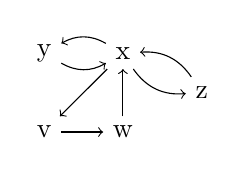
\begin{tikzpicture}

	\node (x) at (0,0) {x};
	\node (y) at (-1,0) {y};
	\node (z) at (1,-0.5) {z};
	\node (v) at (-1,-1) {v};
	\node (w) at (0,-1) {w};

	\path [->] (x) edge[bend right=30] node {} (y);
	\path [->] (y) edge[bend right=30] node {} (x);
	\path [->] (x) edge[bend right=30] node {} (z);
	\path [->] (z) edge[bend right=30] node {} (x);
	\path [->] (w) edge node {} (x);
	\path [->] (v) edge node {} (w);
	\path [->] (x) edge node {} (v);
\end{tikzpicture}
\end{center}
ist stark zusammenhängend.
\begin{center}
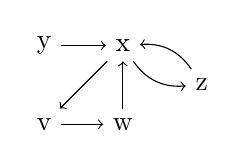
\begin{tikzpicture}

        \node (x) at (0,0) {x};
        \node (y) at (-1,0) {y};
        \node (z) at (1,-0.5) {z};
        \node (v) at (-1,-1) {v};
        \node (w) at (0,-1) {w};

        \path [->] (y) edge node {} (x);
        \path [->] (x) edge[bend right=30] node {} (z);
        \path [->] (z) edge[bend right=30] node {} (x);
        \path [->] (w) edge node {} (x);
        \path [->] (v) edge node {} (w);
        \path [->] (x) edge node {} (v);
\end{tikzpicture}
\end{center}
Dieser Graph, wo der Weg von x nach y entfernt wurde, ist nicht stark zusammenhängend. Die starken Zusammenhangskomponenten sind y und der restliche Graph $G'$.
\end{example}
Im folgenden konstruieren wir einen Algorithmus zur Bestimmung solcher starker Zusammenhangskomponenten.

\begin{algorithm}[H]
\label{alg:starker_zusammenhang}
\caption{Bestimmung starker Zusammenhangskomponenten}
\KwData{Digraph $G=(V,E)$}
\KwResult{Abbildung $comp \colon V \to \N $, welche die Zugehörigkeit zu einer starken Zusammenhangskomponente signalisiert.} 
\begin{itemize}
	\item $R = \emptyset$
	\item $N=0$ 
	\item \For{$v \in V$}{ \If {$v \not\in R$ }{FirstVisit(v)}}
	\item $R = \emptyset$
	\item $K=0$
	\item \For{$j \gets |V|$ \KwTo 1}{{\If{ $\psi^{-1}(j) \not\in R$}{$K=K+1$ \\
		SecondVisit($\psi^{-1}(j)$) } }}	
\end{itemize}
\SetKwFunction{FirstVisit}{FirstVisit}
\SetKwFunction{SecondVisit}{SecondVisit}
 \SetKwProg{Fn}{Function}{}{\KwRet}
\Fn{\FirstVisit{v}{
\begin{itemize}
	\item $R = R \cup \{v\} $ 
	\item \For{$w \in V \setminus R$, $(v,w) \in E$}{FirstVisit(w)}
	\item $N=N+1$ 
	\item $\psi(v)=N$ 
	\item $\psi^{-1}(N)=V$ 
\end{itemize}
}}

\Fn{\SecondVisit{v}{
\begin{itemize}
	\item $R = R \cup \{w\} $ 
	\item \For{$w \in V \setminus R$, $(w,v) \in E$}{SecondVisit(w)}
	\item $comp(v)=K$ 
\end{itemize}
}}

\end{algorithm}

\begin{example}
Wir betrachten den Graph:
\begin{center}
\begin{tikzpicture}

\end{tikzpicture}
\end{center}
Der Startknoten $v_1$ für FirstVisit ergibt die Besuchsreihenfolge: $v_1,v_7,v_2,v_4,v_5$.
Die Tiefensuche mittels FirstVisit bricht für $v_3$ und $v_6$ direkt ab.
Wir erhalten:
\begin{align*}
	\psi(v_2)&=1 & \psi(v_7) &=4 & \psi(v_6)=7 \\
	\psi(v_5)&=2 & \psi(v_1)&=5 \\
	\psi(v_4)&=3 & \psi(v_3)&=6
\end{align*}
SecondVisit für $v_6= \psi^{-1}(7) $ bricht sofort ab $\implies comp(v_6)=1$ \\
SecondVisit für $v_3=\psi^{-1}(6) $ bricht sofort ab $\implies comp(v_3)=2$\\
SecondVisit für $v_1=\psi^{-1}(5)$ ergibt die Besuchsreihenfolge: $v_2,v_7 \implies comp(v_1)=3, v \in \{v_1,v_2,v_7\} $ \\
SecondVisit für $v_4= \psi^{-1}(3)$ ergibt die Besuchsreihenfolge: $v_5 \implies comp(v_4)=4$. 
Demnach ergibt sich:
\[
\{v_6\} , \{v_3\} , \{v_1,v_2,v_7\} , \{v_4,v_5\} 
\]
\end{example}
\begin{theorem}
	Algorithmus \ref{alg:starker_zusammenhang} identifiziert die starken Zusammenhangskomponenten eines Digraphen $G=(V,E)$ in linearem Aufwand $\mathcal{O}(|V|+|E|)$
\end{theorem}
\begin{proof}
	 Aufwand: Analog zur Tiefensuche (Satz \ref{thm:algorithmische_suche})
\begin{itemize}
	\item \underline{Gleiche starke Zusammenhangskomponente $\\implies $ gleicher comp-Wert} \\
Seien $v,w \in V$ Knoten in der gleichen , starken Zusammenhangskomponente \\
\begin{itemize}
	\item $\implies $ Es gibt einen Weg von $v$ nach $w$ und umgekehrt.
	\item $\implies $ SecondVisit weist $comp(v)=comp(w)$ zu
\end{itemize}
\item \underline{Gleicher comp-Wert $\implies $ Gleiche starke Zusammenhangskomponente} \\
Seien $v,w \in V$ mit $comp(v)=comp(w)$. Definiere $r(v)$ ist derjenige von $v$  erreichbare Knoten, der den höchsten $\psi$-Wert hat. \\
\emph{Beobachte:}
\begin{itemize}
	\item $comp(v)=comp(w) \implies v \text{ und } w$  sind im gleichen, von SecondVisist erzeugten Subbaum.
	$\implies r(v)=r(w) \eqqcolon r$ (d.h r ist von $v,w$ erreichbar)
\item $\psi(r)>\psi(v) \implies v$ wurde in FirstVisit vor $r$ nummeriert. $\implies $ Der von FirstVisit erzeugte Baum hat einen Weg von $r$ nach $v$ , d.h $v$ ist von $r$ erreichbar.
\item Analog: $w$ ist von $r$ erreichbar. $\implies v$ ist über $r$ von $w$  aus erreichbar und umgekehrt. 
\end{itemize}
\end{itemize}
\end{proof}
\begin{definition}

\end{definition}
